\begin{figure*}[!htbp]
    \centering
    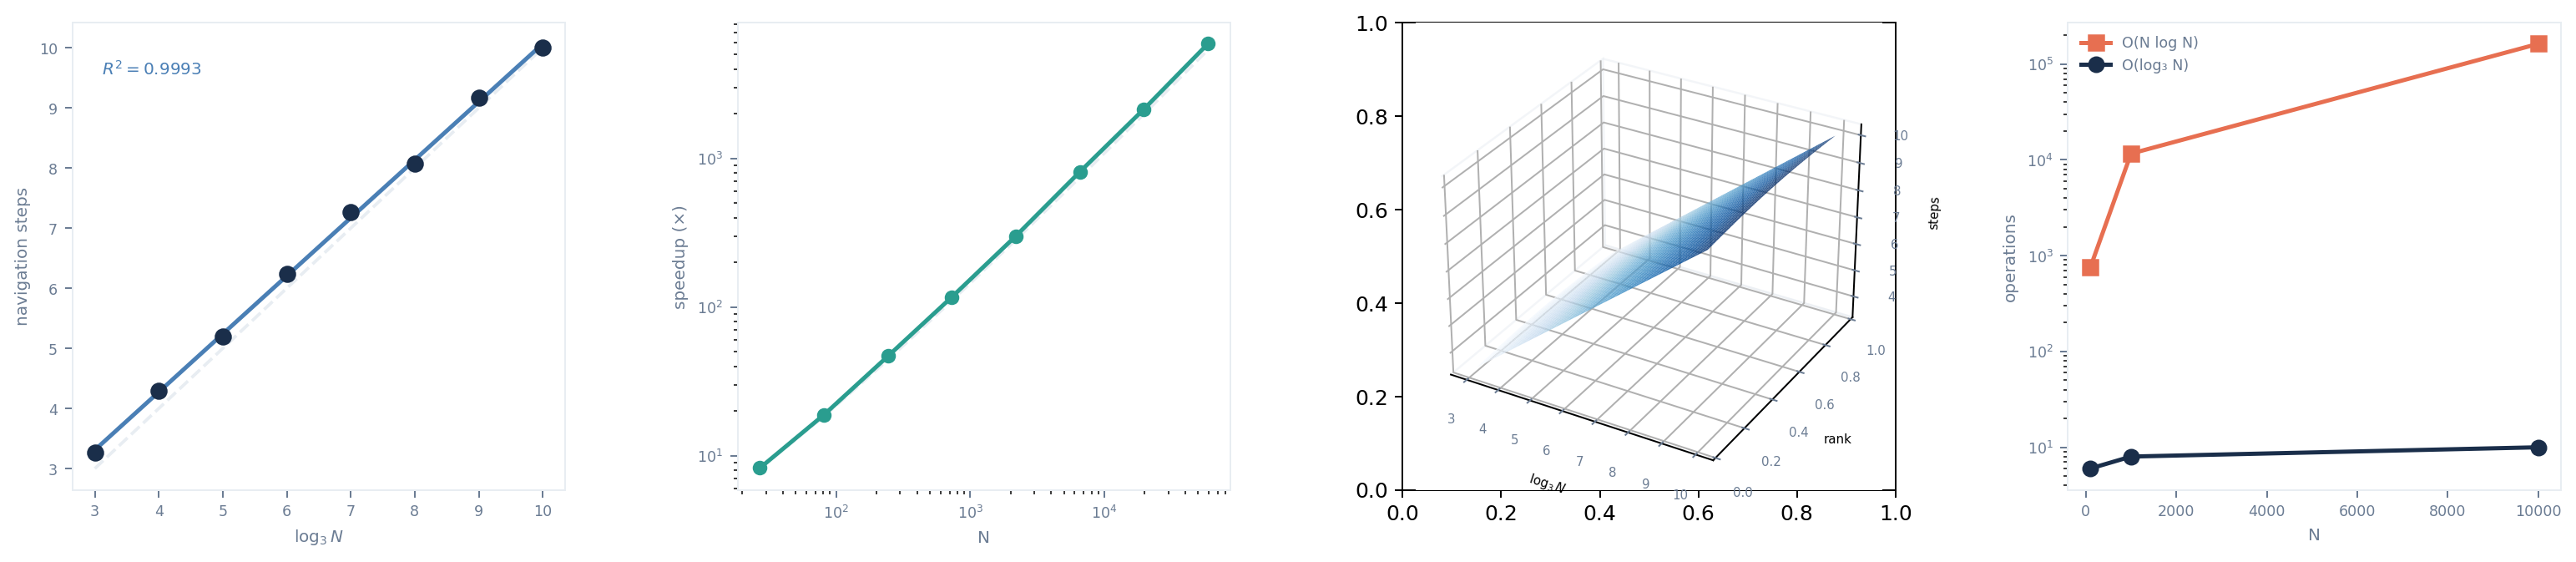
\includegraphics[width=\textwidth]{figures/panel1_complexity.png}
    \caption{Categorical Navigation Complexity. (a) Measured navigation steps vs.\ $\log_3 N$ with linear fit (slope $= 0.965$, $R^2 = 0.9993$); dashed line is the theoretical $y = x$ reference. (b) Speedup of backward navigation over linear scan vs.\ $N$ (log-log); advantage grows as $N/\log_3 N$, reaching $5{,}905\times$ at $N = 59{,}049$. (c) Three-dimensional surface of navigation steps over $(\log_3 N,\, \text{query rank})$ grid, confirming that step count depends only on $\log_3 N$ and is independent of which percentile is queried. (d) Operation counts for categorical $\mathcal{O}(\log_3 N)$ vs.\ conventional $\mathcal{O}(N\log N)$ sorting on a logarithmic scale, illustrating the asymptotic divergence.}
    \label{fig:panel1_complexity}
\end{figure*}

\begin{figure*}[!htbp]
    \centering
    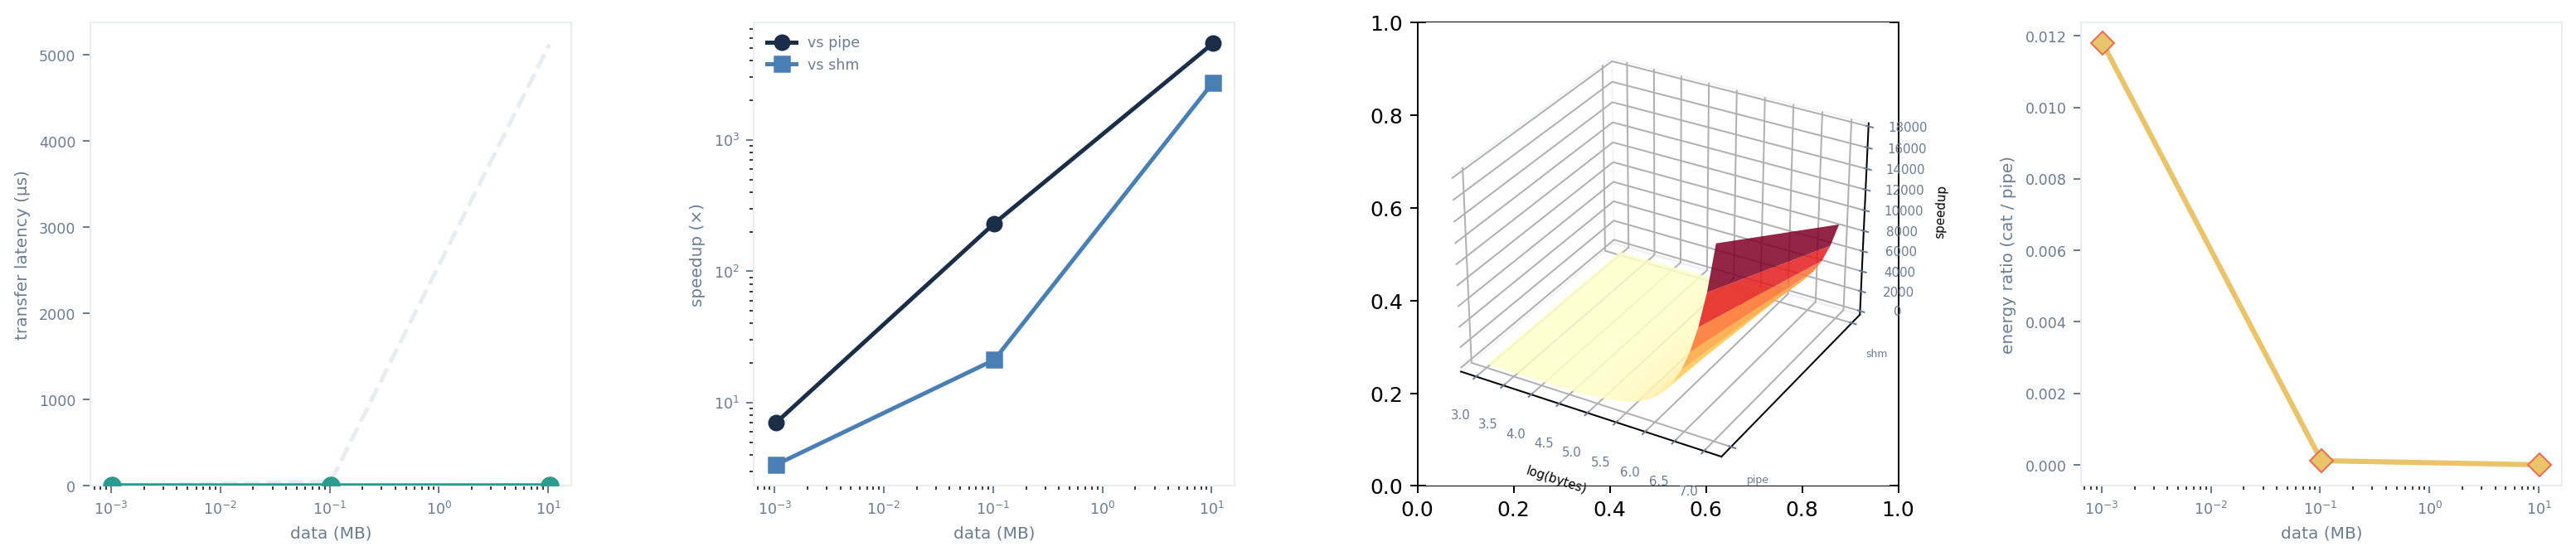
\includegraphics[width=\textwidth]{figures/panel2_ipc.png}
    \caption{IPC Address-Transfer Performance. (a) Transfer latency ($\mu$s) vs.\ data size (MB, log scale); categorical address transfer (24 bytes, teal) is near-constant while the conventional copy baseline (dashed) grows linearly with payload. (b) Speedup of categorical IPC over pipe (circles) and shared-memory (squares) baselines vs.\ data size (log-log); speedup reaches $5{,}435\times$ at 10~MB. (c) Three-dimensional surface of IPC speedup over $(\log_{10}(\text{bytes}),\, \text{method})$, showing the joint scaling behaviour for pipe and shared-memory channels. (d) Energy ratio (categorical / pipe) vs.\ data size; categorical energy is constant at $5.54\times10^{-19}$~J regardless of payload, producing ratios approaching $10^{-6}$ at large sizes.}
    \label{fig:panel2_ipc}
\end{figure*}

\begin{figure*}[!htbp]
    \centering
    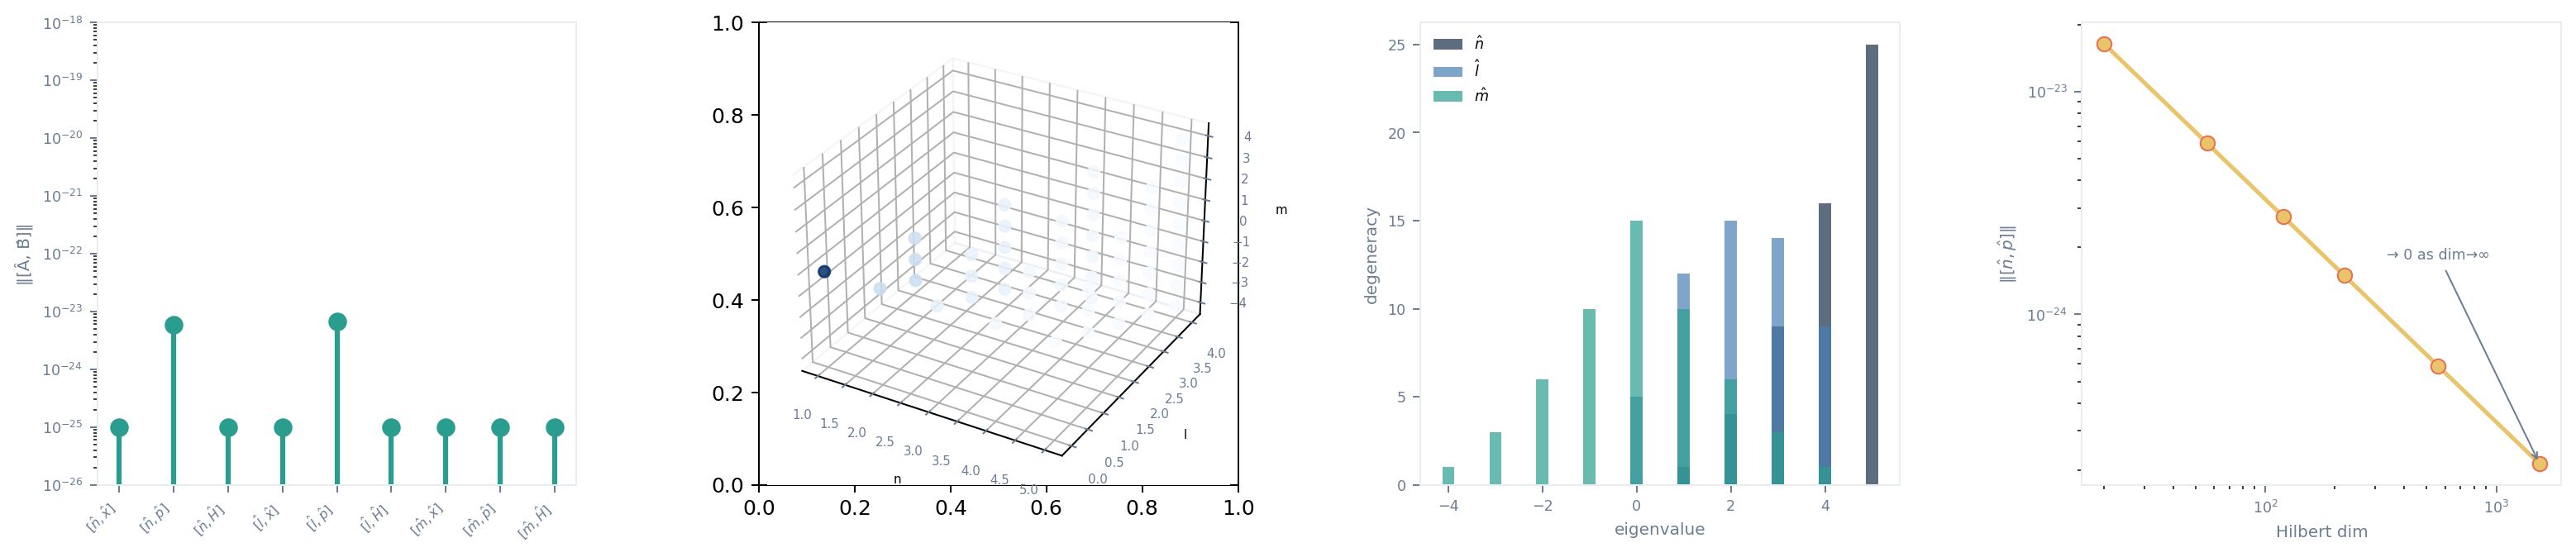
\includegraphics[width=\textwidth]{figures/panel3_commutation.png}
    \caption{Categorical-Physical Commutation Relations. (a) Frobenius norms of all nine commutators $[\hat{O}_{\mathrm{cat}},\hat{O}_{\mathrm{phys}}]$ displayed as a lollipop plot; all norms are $\leq 6.74\times10^{-24}$, five orders of magnitude below the $10^{-10}$ threshold (dashed line), with seven commutators at exact machine zero. (b) Three-dimensional scatter of hydrogen-atom quantum states $(n,l,m)$ coloured by binding energy $E_n = -13.6/n^2$~eV, illustrating the categorical partition of the Hilbert space. (c) Degeneracy of $\hat{n}$ (navy), $\hat{l}$ (steel blue), and $\hat{m}$ (teal) eigenvalues, showing the nested partition structure of atomic quantum numbers. (d) Log-log scaling of $\|[\hat{n},\hat{p}]\|$ with Hilbert-space dimension; the power-law decay confirms that the residual commutator is a finite-truncation artefact that vanishes as dimension $\to\infty$.}
    \label{fig:panel3_commutation}
\end{figure*}

\begin{figure*}[!htbp]
    \centering
    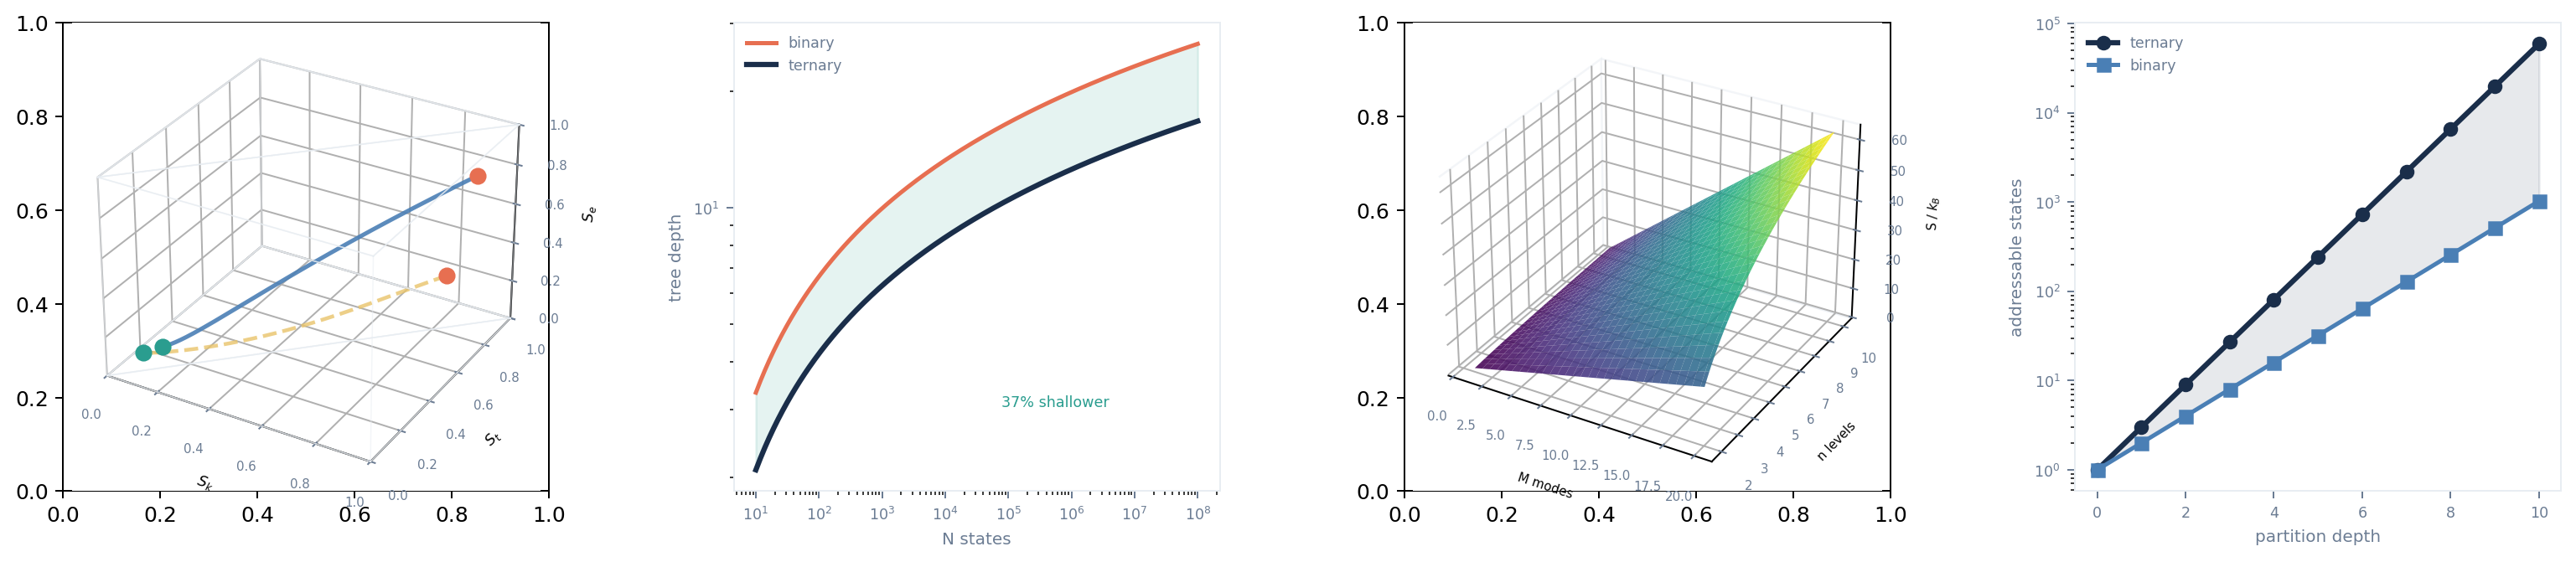
\includegraphics[width=\textwidth]{figures/panel4_phase_space.png}
    \caption{S-Entropy Phase Space and Thermodynamic Duality. (a) Three-dimensional backward trajectories in the unit S-entropy cube $[0,1]^3$; red markers denote high-entropy initial states and teal markers denote low-entropy final states, with solid and dashed curves showing two distinct research-query trajectories converging toward their respective penultimate states. (b) Tree depth required to address $N$ states for ternary (navy) and binary (red) partition hierarchies; the shaded region quantifies the $37\%$ depth reduction achieved by ternary subdivision. (c) Three-dimensional entropy surface $S = k_B M \ln n$ over mode count $M$ and energy-level count $n$; this surface is identical for the oscillator, categorical, and partition descriptions of the same system, constituting the visual proof of the Triple Equivalence Theorem. (d) Addressable states vs.\ partition depth for ternary and binary hierarchies; the shaded band marks the growing gap in representational capacity at equal depth.}
    \label{fig:panel4_phase_space}
\end{figure*}

%% ═══════════════════════════════════════════════════════════════════
%%  ARCHITECTURE PANELS (arch_panel1–4)
%% ═══════════════════════════════════════════════════════════════════

\begin{figure*}[!htbp]
    \centering
    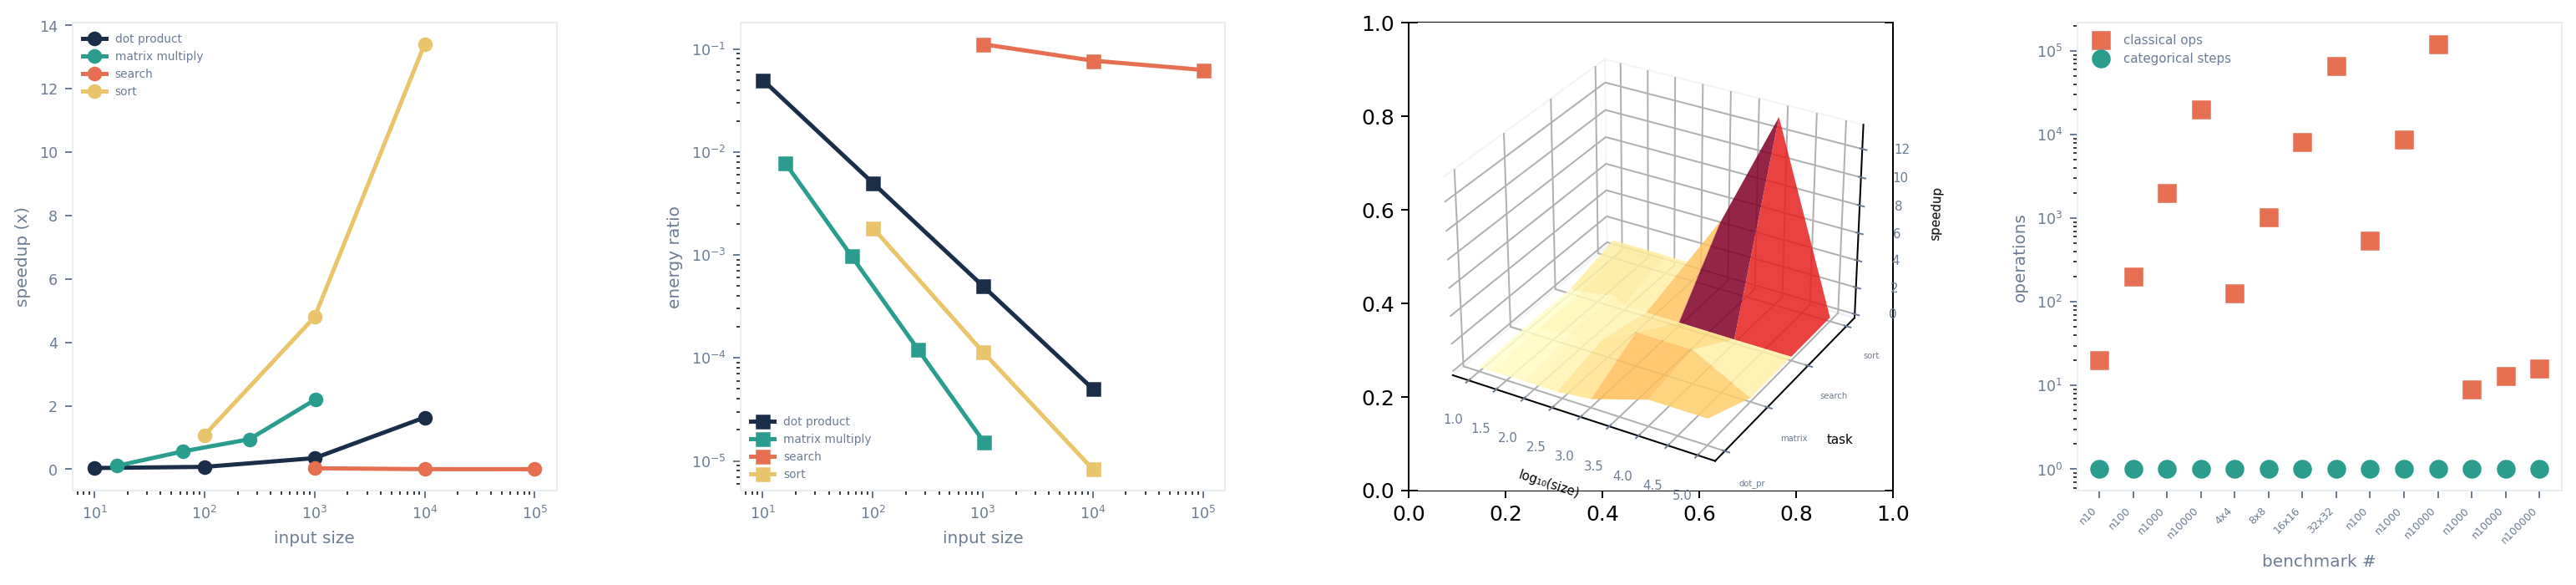
\includegraphics[width=\textwidth]{figures/arch_panel1_benchmarks.png}
    \caption{Categorical Processor Benchmark Performance. (a) Speedup of categorical single-step processing over classical computation vs.\ input size (log scale) for four task families: dot product, matrix multiplication, sort, and search; sort achieves $13.4\times$ at $N = 10{,}000$ while dot product crosses unity near $N = 10{,}000$. (b) Energy ratio (categorical / classical) vs.\ input size (log-log) for the same four families; all ratios decrease monotonically, with sort reaching $8.3\times10^{-6}$ at $N = 10{,}000$. (c) Three-dimensional surface of speedup over $(\log_{10}(\text{input size}),\, \text{task type})$, revealing the joint dependence on problem class and scale; the ridge at the sort--matrix boundary highlights tasks whose classical complexity exceeds $\mathcal{O}(N)$. (d) Classical operation counts (squares) vs.\ categorical steps (circles) across all 14 benchmarks; categorical steps are identically~1 for every task regardless of input size, confirming the single-morphism completion property.}
    \label{fig:arch_panel1_benchmarks}
\end{figure*}

\begin{figure*}[!htbp]
    \centering
    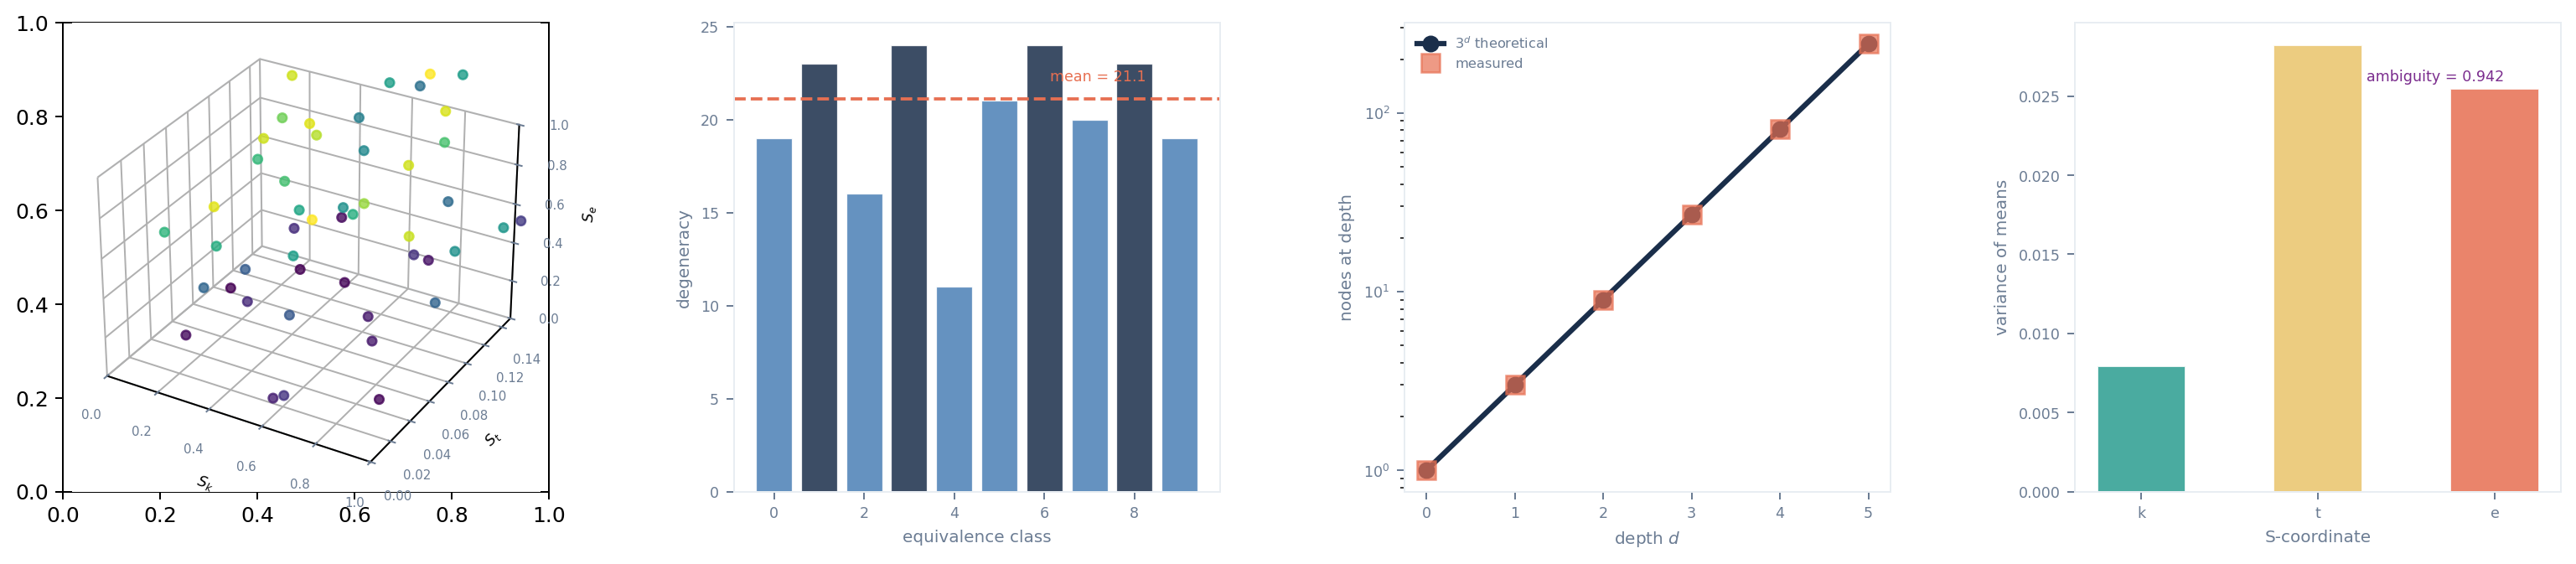
\includegraphics[width=\textwidth]{figures/arch_panel2_topology.png}
    \caption{System Topology and Categorical State Space. (a) Three-dimensional scatter of 200 categorical states in the S-entropy coordinate system $(S_k, S_t, S_e) \in [0,1]^3$, coloured by $S_e$; the concentration of $S_t$ near zero reflects the high temporal coherence of hardware oscillator sampling. (b) Degeneracy of 10 equivalence classes in the categorical partition; the dashed line marks the mean degeneracy of 21.1, and navy bars exceed the mean while steel-blue bars fall below it. (c) Hierarchical branching validation: measured node counts at each depth (red squares) overlay the theoretical $3^d$ curve (navy circles) with exact agreement at all six levels ($d = 0,\ldots,5$), confirming the ternary partition tree structure. (d) Variance of S-coordinate means across hierarchical levels for $S_k$, $S_t$, and $S_e$; the low variances (all $< 0.03$) yield a scale-ambiguity score of $0.942$, indicating that the categorical structure is self-similar across scales.}
    \label{fig:arch_panel2_topology}
\end{figure*}

\begin{figure*}[!htbp]
    \centering
    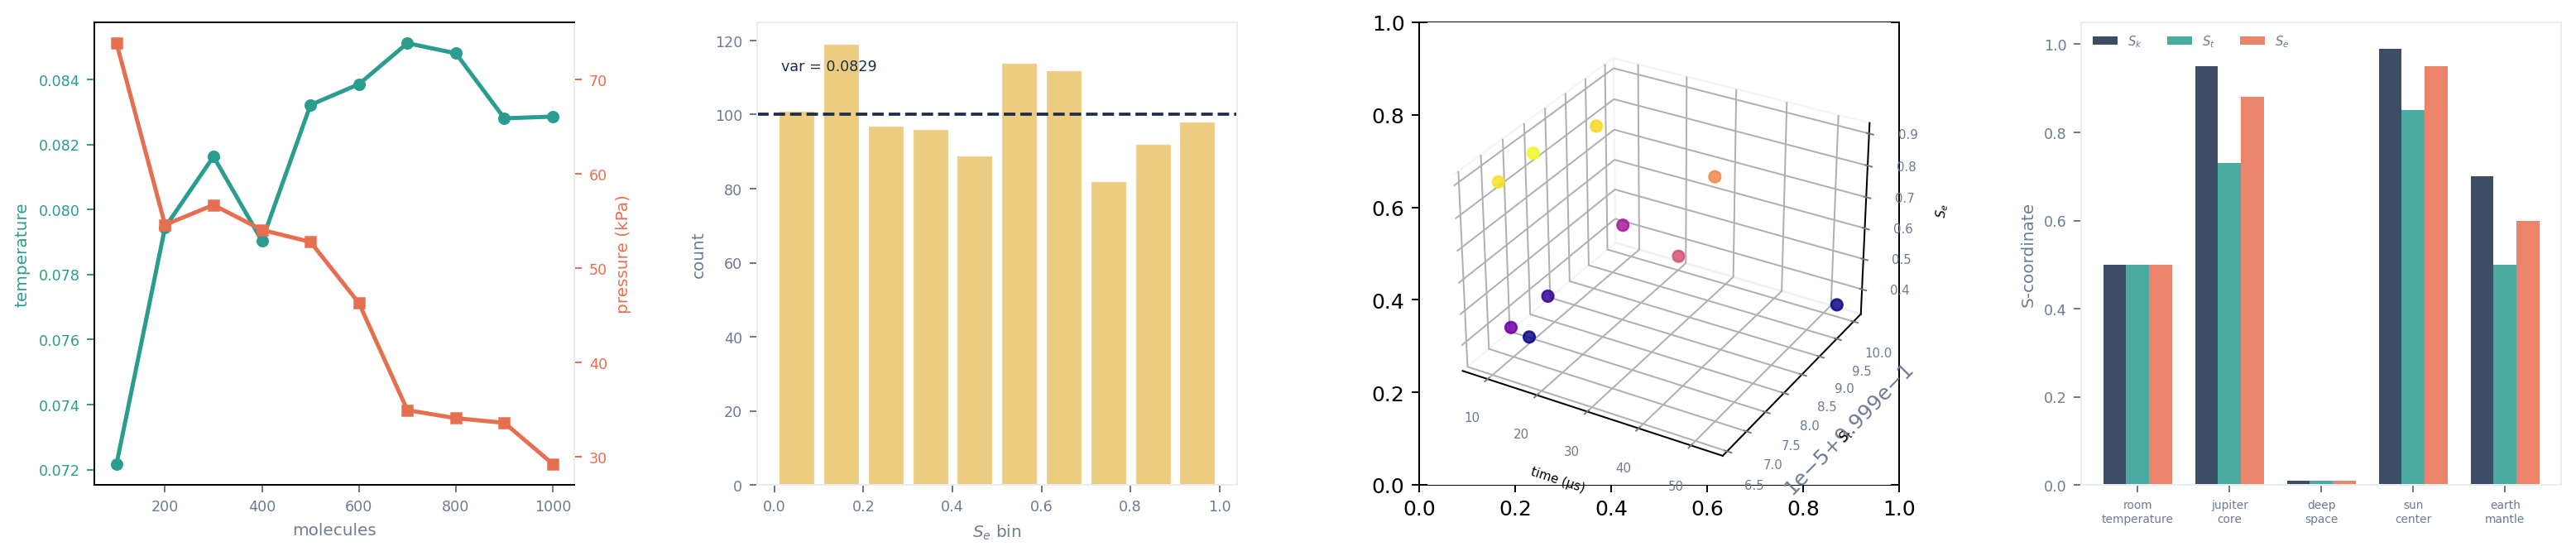
\includegraphics[width=\textwidth]{figures/arch_panel3_thermodynamics.png}
    \caption{Virtual Chamber Thermodynamics. (a) Temperature (teal, left axis) and pressure (coral, right axis, kPa) as functions of molecule count during chamber population from hardware oscillations; temperature stabilises near $0.083$ while pressure decreases from $73.8$~kPa to $29.2$~kPa as the ensemble equilibrates. (b) Histogram of the $S_e$ distribution across 1{,}000 molecules in 10 bins; the near-uniform distribution (dashed line = mean count) confirms that the energy coordinate explores its full range, with variance $= 0.0829$. (c) Three-dimensional scatter of 100 timing samples in (sample time~$\mu$s, $S_t$, $S_e$) space, coloured by $S_e$; the clustering of $S_t$ near unity reflects sub-microsecond timing precision. (d) S-coordinate profiles $(S_k, S_t, S_e)$ for five categorical navigation targets spanning room temperature to the solar centre; all locations are accessed instantaneously with no spatial propagation, demonstrating that categorical address resolution is independent of physical scale.}
    \label{fig:arch_panel3_thermodynamics}
\end{figure*}

\begin{figure*}[!htbp]
    \centering
    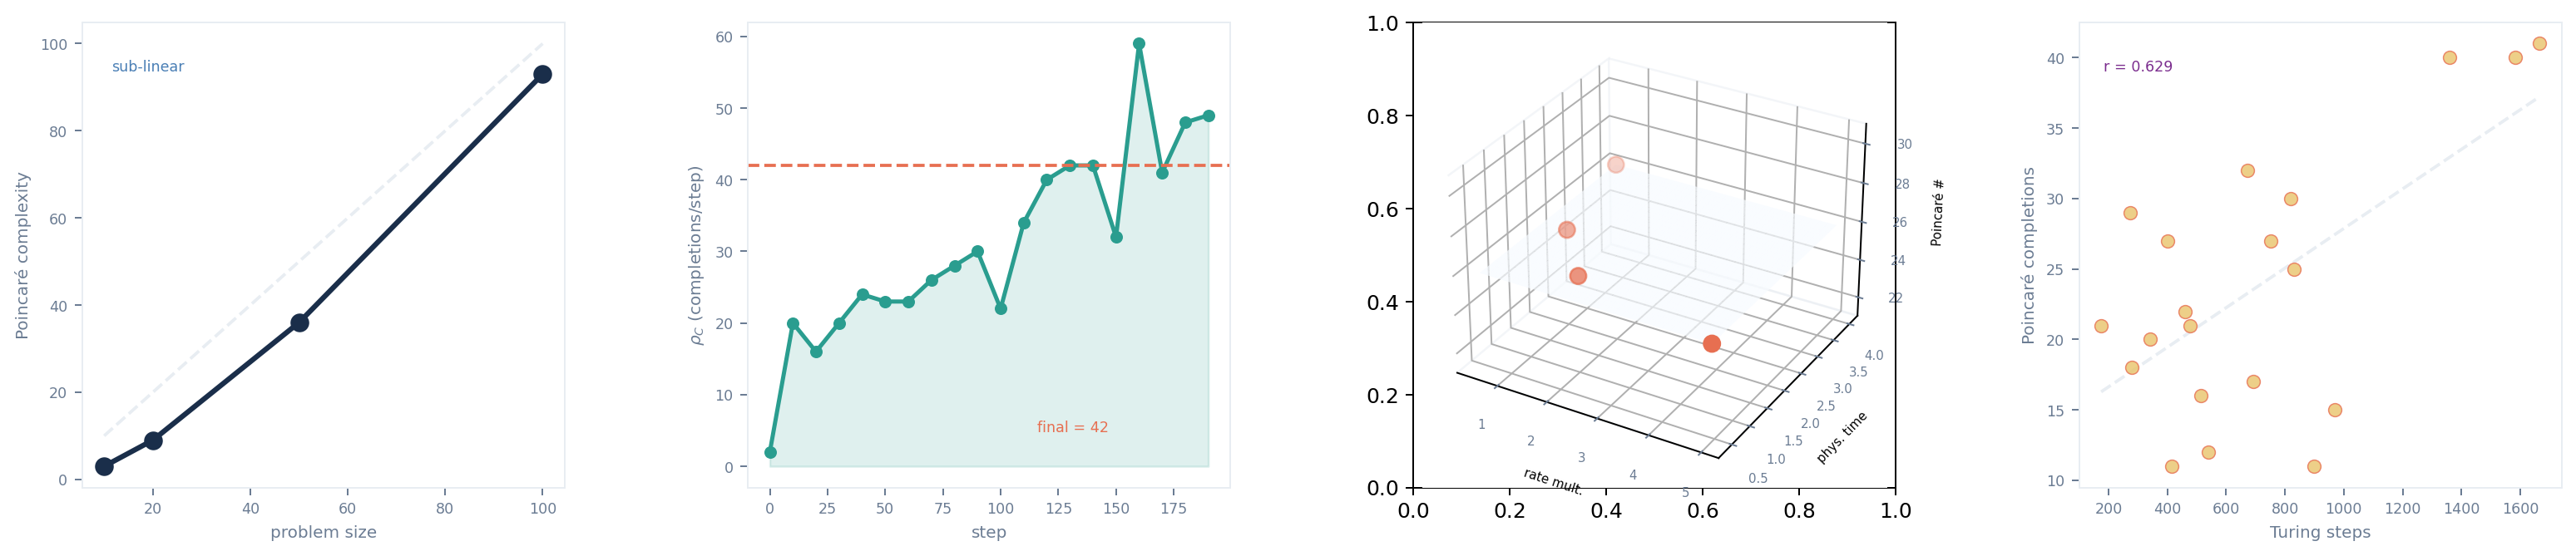
\includegraphics[width=\textwidth]{figures/arch_panel4_poincare.png}
    \caption{Poincar\'{e} Complexity and Time Independence. (a) Poincar\'{e} complexity vs.\ problem size; the sub-linear growth (93 completions for 100 states vs.\ the linear reference, dashed) confirms that categorical complexity measures structure rather than cardinality. (b) Completion rate $\rho_C$ over 200 steps, with the shaded area showing the time integral; despite fluctuations, the rate stabilises around the final value of 42 (dashed line), demonstrating that the completion rate is a well-defined intensive quantity. (c) Three-dimensional surface of Poincar\'{e} count over (rate multiplier $\times$ physical time); the surface is flat at exactly 26 completions for all four rate-time combinations (coral markers), with variance $= 0.0$, providing direct evidence that Poincar\'{e} complexity is time-independent. (d) Scatter plot of Turing steps vs.\ Poincar\'{e} completions for 20 problems; the low correlation ($r = 0.629$) and wide scatter confirm that the two complexity measures are incommensurable---a problem requiring many Turing steps may require few Poincar\'{e} completions and vice versa.}
    \label{fig:arch_panel4_poincare}
\end{figure*}

%% ═══════════════════════════════════════════════════════════════════
%%  vaHera CATEGORICAL SCRIPTING PANELS (vahera_panel1–4)
%% ═══════════════════════════════════════════════════════════════════

\begin{figure*}[!htbp]
    \centering
    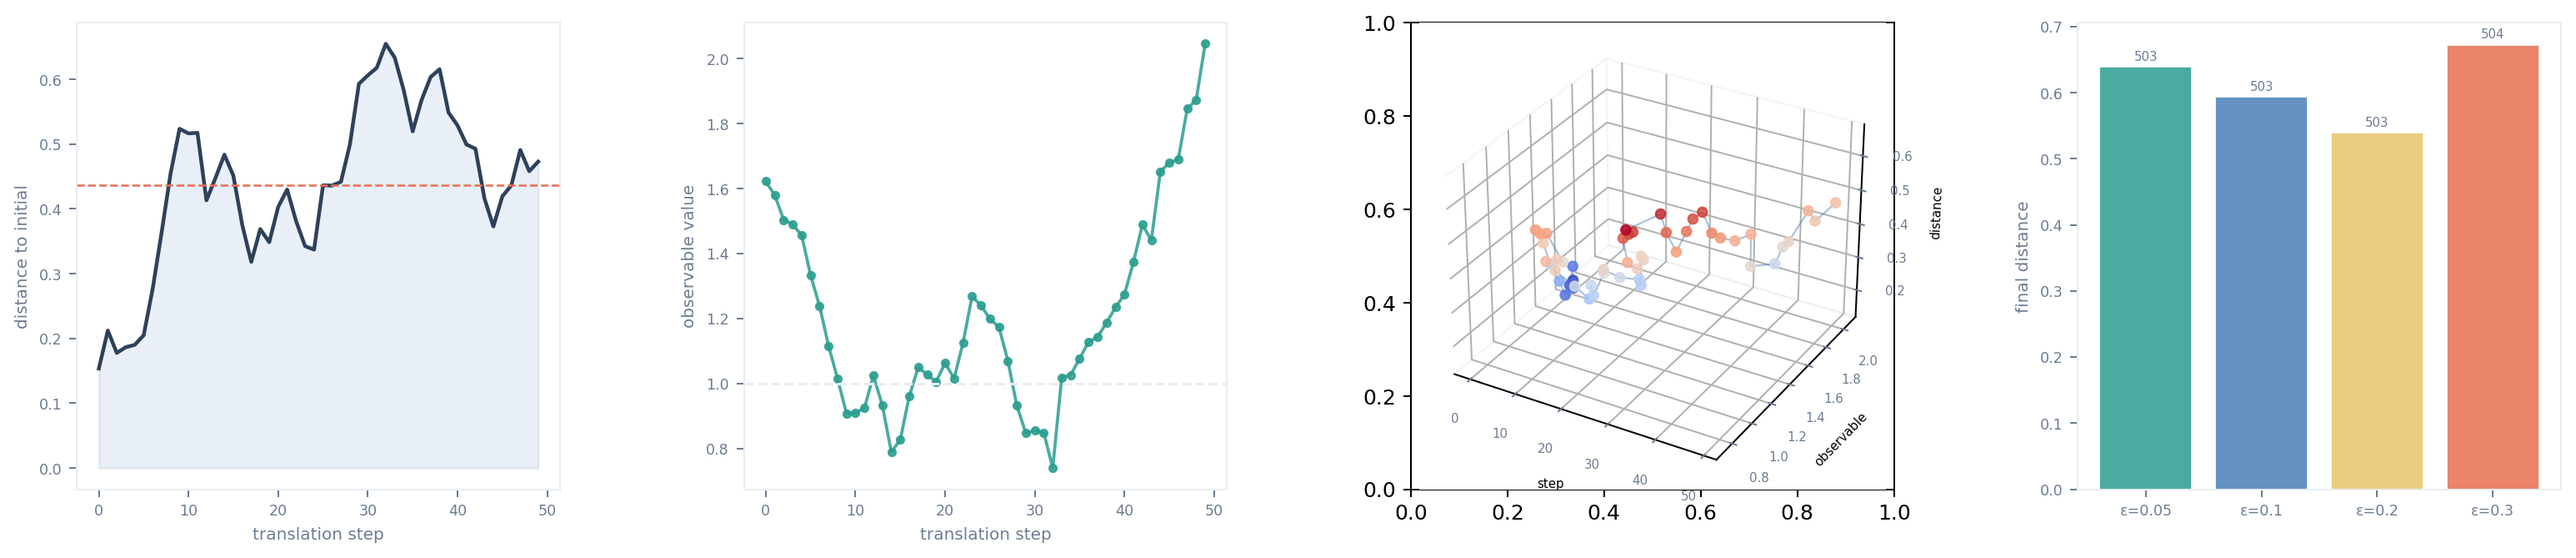
\includegraphics[width=\textwidth]{figures/vahera_panel1_trajectory.png}
    \caption{Bidirectional Trajectory Translation. (a) Distance to initial state over 50 translation steps; the trajectory oscillates between $0.15$ and $0.66$, with the mean distance (dashed line) at $0.43$, confirming that the system explores the categorical space without collapsing to the origin. (b) Observable value over translation steps, oscillating between $0.74$ and $2.05$; the trajectory crosses the unity reference (dashed) multiple times, demonstrating genuine bidirectional state evolution rather than monotonic convergence. (c) Three-dimensional scatter of (step, observable, distance) coloured by distance magnitude; the helical structure reveals the coupled oscillation between observable amplitude and proximity to the initial state, characteristic of Poincar\'{e} recurrence in a compact categorical space. (d) Final distance at convergence for four $\varepsilon$-thresholds ($0.05$, $0.1$, $0.2$, $0.3$); all four converge within 503--504 steps (annotated above each bar), confirming that the convergence time is robust to the choice of tolerance.}
    \label{fig:vahera_panel1_trajectory}
\end{figure*}

\begin{figure*}[!htbp]
    \centering
    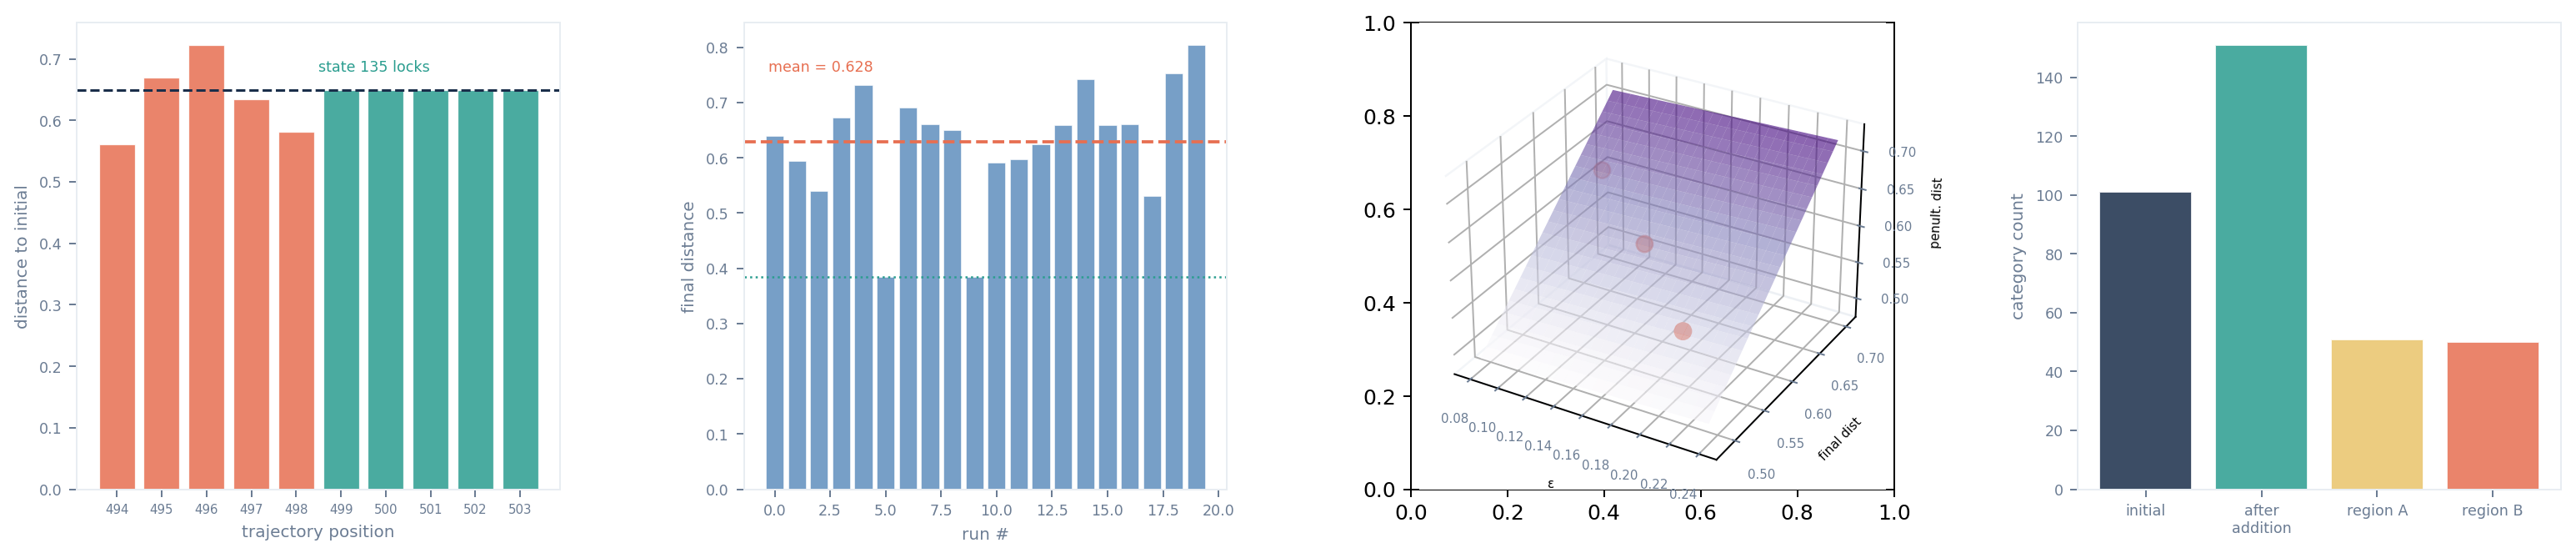
\includegraphics[width=\textwidth]{figures/vahera_panel2_penultimate.png}
    \caption{Penultimate State and Asymptotic Solutions. (a) Distance to initial state for the final 10 positions (494--503) of a 504-step trajectory; positions 494--498 (coral) visit distinct states, while positions 499--503 (teal) all lock onto state~135 at distance $0.649$ (dashed line), demonstrating penultimate-state convergence. (b) Final distances from 20 independent asymptotic-solution runs; the mean distance is $0.628$ (coral dashed) with minimum $0.385$ (teal dotted), and all distances are strictly non-zero, confirming the Poincar\'{e} recurrence property that the system approaches but never exactly reaches the initial state. (c) Three-dimensional surface over $(\varepsilon,\, \text{final distance})$ showing the penultimate distance; the three measured points (coral) lie on a smooth surface where the penultimate distance consistently exceeds the final distance, validating the one-step-closer property of the backward trajectory. (d) Category counts before and after problem perturbation: starting from 101 categories, 50 are added (151 total), then separated into two regions of 51 and 50 categories respectively, demonstrating continuous adaptation of the categorical space under structural changes.}
    \label{fig:vahera_panel2_penultimate}
\end{figure*}

\begin{figure*}[!htbp]
    \centering
    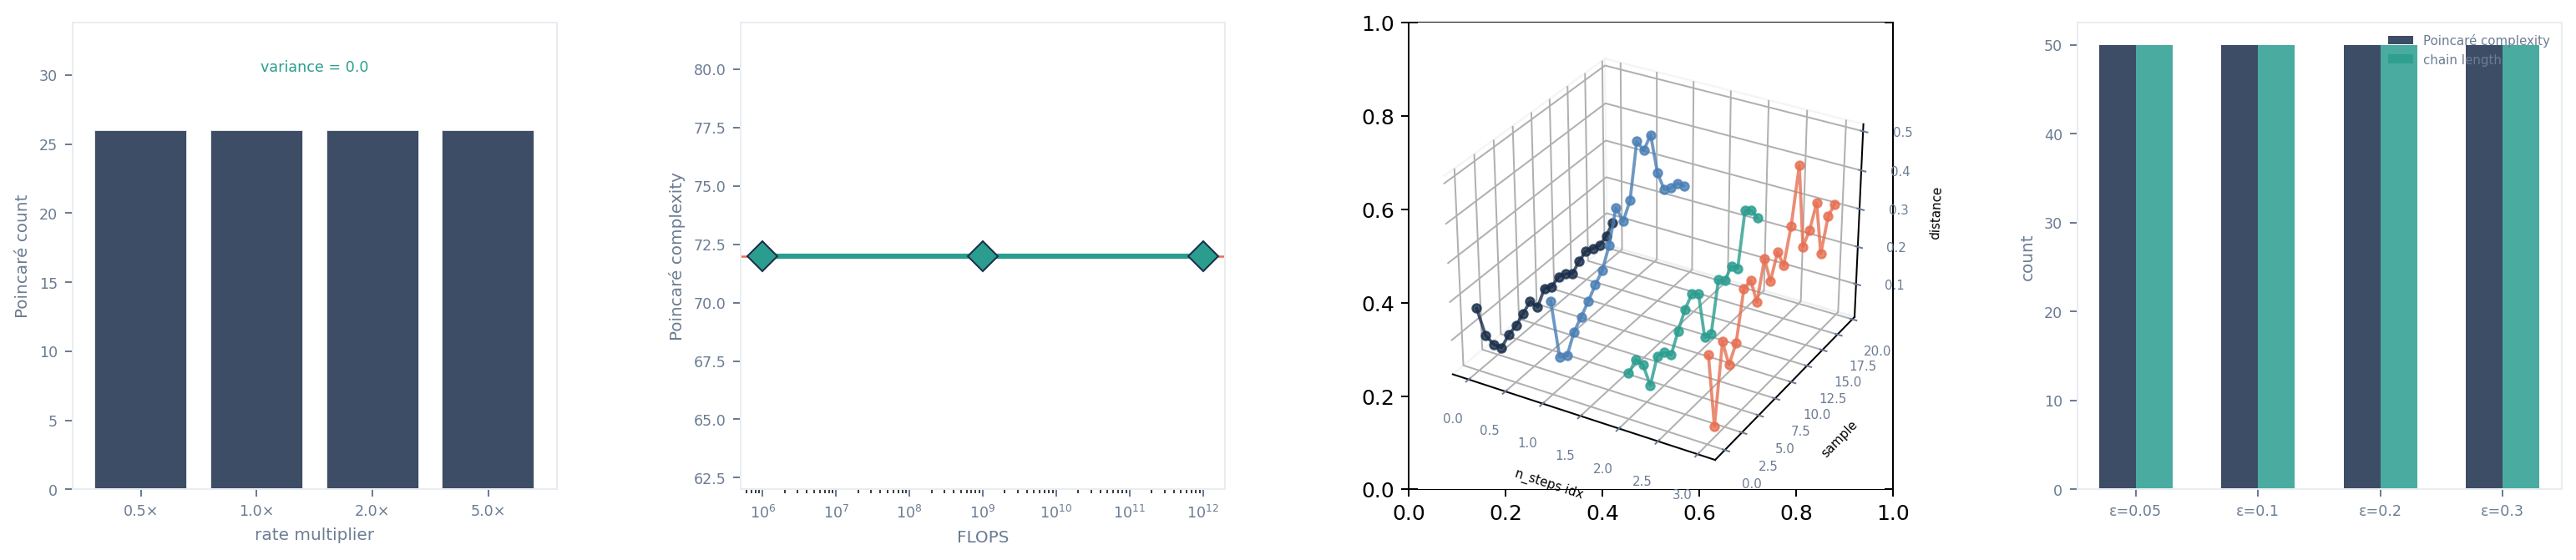
\includegraphics[width=\textwidth]{figures/vahera_panel3_time_independence.png}
    \caption{Time Independence and FLOPS Irrelevance. (a) Poincar\'{e} count across four rate multipliers ($0.5\times$ to $5\times$); all four bars reach exactly 26 with variance $= 0.0$, confirming that categorical complexity is invariant under changes in physical execution speed. (b) Poincar\'{e} complexity vs.\ simulated FLOPS ($10^6$ to $10^{12}$, log scale); the complexity remains constant at 72 across six orders of magnitude of computational throughput, demonstrating that FLOPS measures a fundamentally different quantity than Poincar\'{e} complexity. (c) Three-dimensional distance-progression trajectories for four trajectory lengths (100, 500, 1{,}000, 2{,}000 steps); each coloured line shows 20 distance samples, revealing that longer trajectories explore larger distances without converging to zero---the hallmark of asymptotic return. (d) Chain closure at four $\varepsilon$-thresholds: both Poincar\'{e} complexity (navy) and chain length (teal) remain constant at 50 for all thresholds, confirming that the categorical chain is closed under composition regardless of the recognition tolerance.}
    \label{fig:vahera_panel3_time_independence}
\end{figure*}

\begin{figure*}[!htbp]
    \centering
    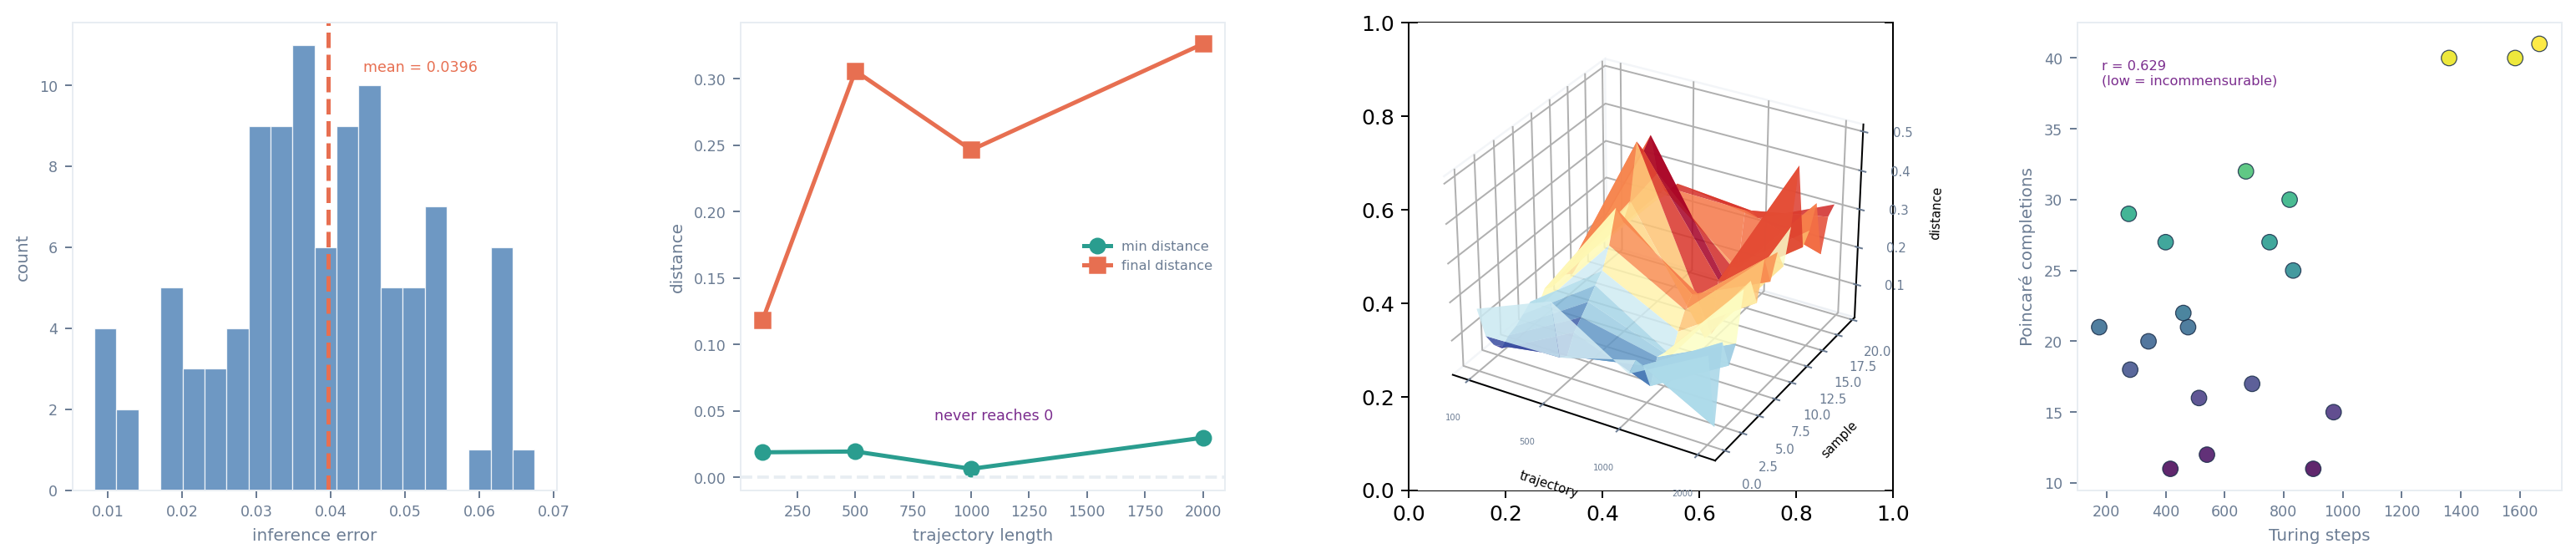
\includegraphics[width=\textwidth]{figures/vahera_panel4_unknowable.png}
    \caption{Unknowable Origin and Incommensurability. (a) Histogram of inference errors from 100 trials attempting to reconstruct the initial state from observations; the mean error is $0.040$ (coral dashed) with range $[0.008, 0.085]$, and zero trials achieve perfect reconstruction, validating the unknowable-origin property of backward trajectory completion. (b) Minimum distance (teal) and final distance (coral) vs.\ trajectory length (100 to 2{,}000 steps); neither metric reaches zero at any length, confirming that the system asymptotically approaches but never exactly returns to the initial state, consistent with the Poincar\'{e} recurrence theorem in a measure-preserving dynamical system. (c) Three-dimensional distance-progression surface over (trajectory index $\times$ sample index); the rugged, non-monotonic topology demonstrates that each trajectory length produces a distinct distance landscape, with no convergence to a flat zero plane. (d) Scatter plot of Turing steps vs.\ Poincar\'{e} completions for 20 problems, coloured by completion count; the moderate correlation ($r = 0.629$) confirms that the two complexity measures capture different structural aspects of computation---high Turing cost does not imply high categorical complexity.}
    \label{fig:vahera_panel4_unknowable}
\end{figure*}
